\chapter{Complete coverage path planning} \label{ch:ccpp}

%Sensors, SLAM, Partitioning, CCPP

Complete coverage path planning is the task of determining a collision-free feasible path such that a sensor or end-effector passes over all points of an area of interest. Chapter \ref{ch:slam} explained how information gathered from the sensors are fused with SLAM in order to give accurate localization of the USV and a 2D mapping of its surroundings. In Chapter \ref{ch:partition}, this information was used with partitioning methods in order to create a workspace representation more useful for path planning. In this chapter, two CCPP methods are presented which makes use of these partitions. Section \ref{sec:ccpp_binn} presents a method that uses a topologically organized neural network to determine the path, and Section \ref{sec:ccpp_ba} describes a method based on boustrophedon motions and the A* search algorithm. 

\section{Bio-inspired neural network} \label{sec:ccpp_binn}

This method uses the circular cell partitioning described in Section \ref{sec:circle_partition}.

\subsection{Neural network model}

In \citet{yang2004neural}, a neural network architecture is developed for CCPP where the dynamic neural activity landscape represents the dynamically varying environment of a robot. This neural network is designed such that uncovered areas stay at the peaks of the neural network, while areas with obstacles stay in the valleys. Moreover, uncovered areas globally attract through neural activity propagation, while areas with obstacles only locally push away.

For each circular cell in the workspace partition, associate a neuron $x_i \in \mathbb{R}$. Each neuron $x_i$ then has a position $p_i \in \mathbb{R}^2$ which is at the center of the associated cell. Given the position $p_i$, the set of neighboring neurons can then be defined as
\begin{equation}
\text{neig}_{r_0}(p_i) = \{p_j|\ |p_i-p_j| \leq r_0\}
\end{equation}
where $r_0 > 0$ is a constant determining the size of the neighborhood, and $|p_i-p_j|$ is the Euclidean distance between two neurons with positions $p_i$ and $p_j$. The 2D architecture of the network can be seen in \figref{fig:arch_nn}.

\begin{figure}[h!]
	\centering
	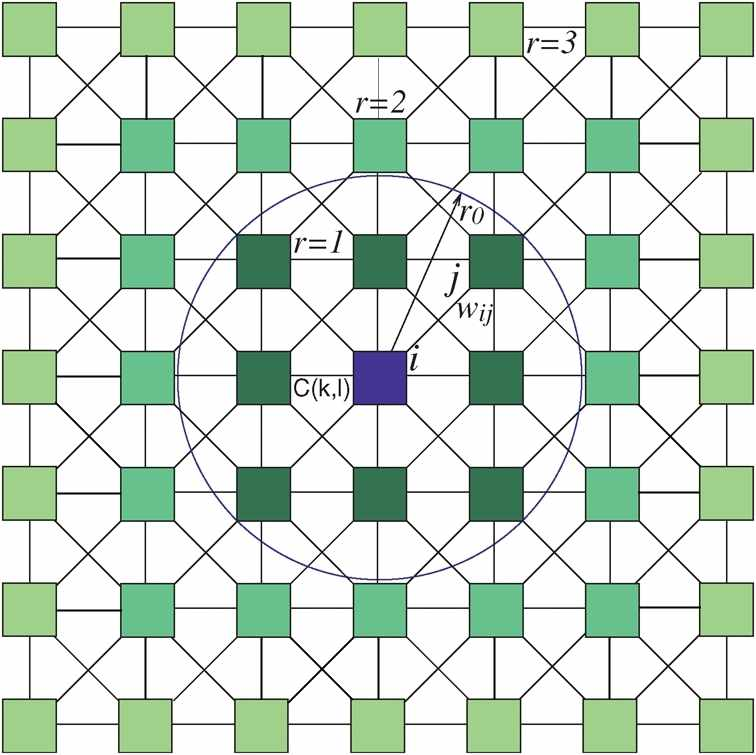
\includegraphics[width=0.5\textwidth]{fig/ccpp/nn_architecture2}
	\caption[Architecture of the 2D neural network.]{Architecture of the 2D neural network \citep{luo2008bioinspired}.}
	\label{fig:arch_nn}
\end{figure}

The dynamic activity of the $i$th neuron can be characterized by \citep{yang2004neural}
\begin{equation} \label{eq:binn}
\dot{x_i} = -A x_i + (B - x_i)\left([I_i]^{+} + \sum^k_{j=1}w_{ij}[x_j]^{+} \right) - (D+x_i)[I_i]^{-}
\end{equation}
where $A$, $B$, and $D$ are non-negative constants representing the passive decay rate and the upper and lower bounds of the neuron, i.e. $x_i \in [-D, B]$. $I_i$ is the external input to the $i$th neuron which can be defined as \citep{Scibilia2012}
\begin{equation}
I_i = 
\begin{cases}
\lambda_i E, & \text{if it is an unvisited area} \\
-E, & \text{if it is an obstacle area} \\
0, & \text{otherwise}
\end{cases}
\end{equation}
where $0 < \lambda_i \leq 1$ are scaling factors that can be used to prioritize certain areas, and $E$ is a constant such that $\lambda_i E \gg B$. The functions $[a]^{+}$ and $[a]^{-}$ are defined as $[a]^{+} = \max\{a,0\}$ and $[a]^{-} = \min\{-a,0\}$. $k$ is the number of neighboring neurons, and $x_j$ is a neuron in the neighborhood of $x_i$, i.e. $p_j \in \text{neig}_{r_0}(p_i)$. $w_{ij}$ is the connection weight between the $i$th and $j$th neuron defined as 
\begin{equation}
w_{ij} = \frac{\mu}{|p_i-p_j|}
\end{equation}
where $\mu > 0$ is a tuning constant. 

The neural connections $w_{ij}$ are defined in the design stage. Therefore, this neural network does not require any learning procedures. Neural connections only exist in the excitatory input $\left([I_i]^{+} + \sum^k_{j=1}w_{ij}[x_j]^{+} \right)$ in \eqref{eq:binn}. This means only positive neural activity can propagate. Consequently, uncovered areas globally attract, while obstacles only locally push away.

\subsection{Using the neural network for path planning}

Positive neural activity represents free uncovered areas. Deciding where to go next can then simply be done by going towards the most positive neuron at all times. Given the current position $p_q$ and heading $\theta_q$, \citet{Scibilia2012} suggest choosing the next position $p_n$ as
\begin{equation} \label{eq:binn_pos}
p_n \Leftarrow x_n = \argmax_{x_j:\ p_j \in \text{neig}_{r_0}(p_q)} \left\{ \left( 1 - \frac{\text{diff}(\theta_q,\theta_j)}{\pi} \right)\lambda x_j + (1-\lambda)x_j \right\}
\end{equation}
where $0 \leq \lambda \leq 1$ is a tuning constant which can be used to prioritize areas that do not require a change of direction. The function $\text{diff}(\theta_q,\theta_j)$ measures the smallest angle difference between $\theta_q$ and $\theta_j$. $\theta_j$ is the angle of the USV when it reaches $p_j$, and should be determined by the feasible path generation strategy employed. In this thesis, that means $\theta_j$ is the angle at the end of a simple Dubins path constructed from $p_q$ and $\theta_q$ to $p_n$. The computation of this angle is described in Section \ref{sec:pathgen}.

Complete coverage is then achieved by following the steps summarized in Algorithm 1. The steps are slightly modified from the algorithm presented in \citet{Scibilia2012} in order to incorporate the changes of \citet{luo2008bioinspired} and make it work for completely unknown environments.

\begin{tcolorbox}

\textbf{Algorithm 1: CCPP with bio-inspired neural network}

\emph{Input: Pose of USV, and rolling window map}

\begin{enumerate}
\itemsep0em

\item Partition the workspace into circular cells as described in Section \ref{sec:circle_partition}. Set the status of each cell to unknown, and mark all cells as uncovered.

\item Associate a neuron to each cell in the partition, and set all neural activities to zero.

\item Update the status of cells nearby the USV with information from the rolling window of Section \ref{sec:map_processing}.

\item If no reachable free cells remain, terminate the algorithm. Complete coverage has then been achieved. Else, continue with the substeps.
\begin{enumerate}
\itemsep0em

\item Update the status of cells nearby the USV with information from the rolling window of Section \ref{sec:map_processing}.

\item Evolve the neural network as in \eqref{eq:binn}.

\item Find next position as in \eqref{eq:binn_pos}. If the found next position is the same as the current position, stay still.

\item Mark the cell corresponding to the current position as covered.

\end{enumerate}

\item Go to step 4.

\end{enumerate}

\end{tcolorbox}


\section{Boustrophedon motions} \label{sec:ccpp_ba}

The proposed method solves the online complete coverage task in unknown workspaces using boustrophedon motions (i.e. a back-and-forth lawnmower pattern) and the A* search algorithm. The method works by first performing a boustrophedon motion in an uncovered region until a critical point is reached, i.e. a point where all nearby points are already covered or blocked by obstacles. To find a new uncovered region to cover, the method intelligently detects backtracking points based on accumulated knowledge. The best backtracking point is chosen as the starting point of the next boustrophedon motion, and an A* search is performed in order to reach the next starting point with the shortest collision-free path possible. When no backtracking points are detected, complete coverage is achieved. The usage of backtracking points is based on the work by \citet{Viet2013}, and minimizes the required number of boustrophedon motions before complete coverage is achieved. This method uses the square cell partitioning described in Section \ref{sec:square_partition}.

\subsection{Constructing the boustrophedon motion}

Collision-free motion is achieved by moving from one free cell to a neighboring free cell in the partition. When performing a boustrophedon motion, the algorithm's motion in the grid is defined by its moving direction (north or south) and its sweeping direction (east or west). The algorithm will start by moving straight forward in the moving direction until the next position is either blocked, or everything inside the coverage range is already covered. The boustrophedon motion is illustrated in \figref{fig:bm_dir}.

When the algorithm can no longer move straight forward it will try to perform wall following. If there are uncovered free cells in the sweeping direction, the algorithm will perform wall following in the sweeping direction. If no uncovered free cells are found, the sweeping direction is switched: from east to west or from west to east. Wall following is then attempted again in the new sweeping direction. If the algorithm still cannot find uncovered free cells, a critical point has been reached and the algorithm backtracks if possible.

If the algorithm decides to wall follow, it will move in the sweeping direction twice the number of cells covered by the shortest coverage range on the current lap.
For example, if the algorithm detects a wall after moving north with a coverage range that varies between 3 and 4 cells, the algorithm will wall follow 6 cells in the sweeping direction. This approach to variable inter-lap spacing is inspired by \citet{galceran2012efficient}, and minimizes the overlapping sensor coverage. When the desired number of cells is reached, or the algorithm is blocked from moving further, wall following is finished. The moving direction is then switched: from north to south or from south to north, and the algorithm starts on a new lap. The boustrophedon motion is summarized in Algorithm 2.

\begin{figure}[h!]
	\centering
	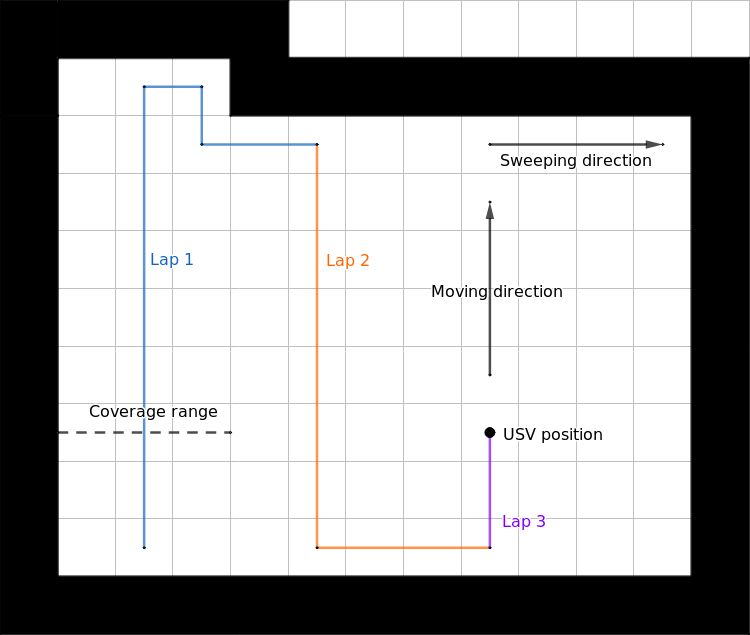
\includegraphics[width=0.5\textwidth]{fig/ccpp/bm_desc}
	\caption[Boustrophedon motion with a symmetric constant coverage range.]{Boustrophedon motion with a symmetric constant coverage range. White cells are free and black cells are obstacles.}
	\label{fig:bm_dir}
\end{figure}

\begin{tcolorbox}

\textbf{Algorithm 2: Constructing a boustrophedon motion}

\emph{Input: Pose of USV, coverage range, partitioned workspace, and rolling window map}

\begin{enumerate}
\itemsep0em

\item Check one step along the moving direction.
\begin{enumerate}
\itemsep0em

\item If the cell is free and the current coverage range ensures that new cells are covered by moving to it: move one cell along this direction. Then go to step 2. Else, continue.

\item If the cell is blocked and uncovered free cells are available in the sweeping direction: wall follow one cell in the sweeping direction. Then go to step 2. Else, continue.

\item If the cell is blocked and uncovered free cells are available opposite of the sweeping direction: switch sweeping direction and wall follow one cell in the new sweeping direction. Then go to step 2. Else, continue.

\item A critical point has been reached. Terminate the algorithm.

\end{enumerate}
\itemsep0em

\item Mark cells as covered based on the coverage range and method of Section \ref{sec:handle-mbes}.

\item Update the status of cells nearby the USV with information from the rolling window of Section \ref{sec:map_processing}. Go to step 1.

\end{enumerate}

\end{tcolorbox}



\subsection{Determining the backtracking point}

Complete coverage most often requires multiple boustrophedon motions. After finishing a motion, a backtracking point needs to be determined as the starting point of the next boustrophedon motion. This can generally be at any free uncovered cell in the grid map. However, choosing the next starting point wisely can reduce the amount of boustrophedon motions required to achieve complete coverage. \citet{Viet2013} therefore suggest a strategy of choosing candidate backtracking points where the surrounding 8 cells are considered. Let $s_i$ with $i=1,2,...8$ be the surrounding cells as in \figref{fig:bps}. A backtracking point is then detected if $\mu (s) \geq 1$ where
\begin{multline} \label{eq:bp1}
\mu (s) = b(s_1,s_8)+b(s_1,s_2)+b(s_3,s_2)+b(s_3,s_4)+b(s_5,s_6) \\ 
+b(s_5,s_4)+b(s_7,s_6)+b(s_7,s_8)
\end{multline}
and
\begin{equation} \label{eq:bp2}
b(s_i,s_j) = 
\begin{cases}
1, & \text{if ($s_i$ is free) and ($s_j$ is blocked)} \\
0, & \text{otherwise.}
\end{cases}
\end{equation}
Note that \eqref{eq:bp1} is modified to also include $s_3$, since the proposed method does not use the same north-south-east-west priority as \citet{Viet2013}. Among these candidates, the backtracking point is chosen as the candidate with the shortest distance to the current critical point. In this thesis, the backtracking point with the shortest path using an A* search is chosen. If no backtracking points are found, complete coverage is achieved and the method is finished. 

\begin{figure}[h!]
	\centering
	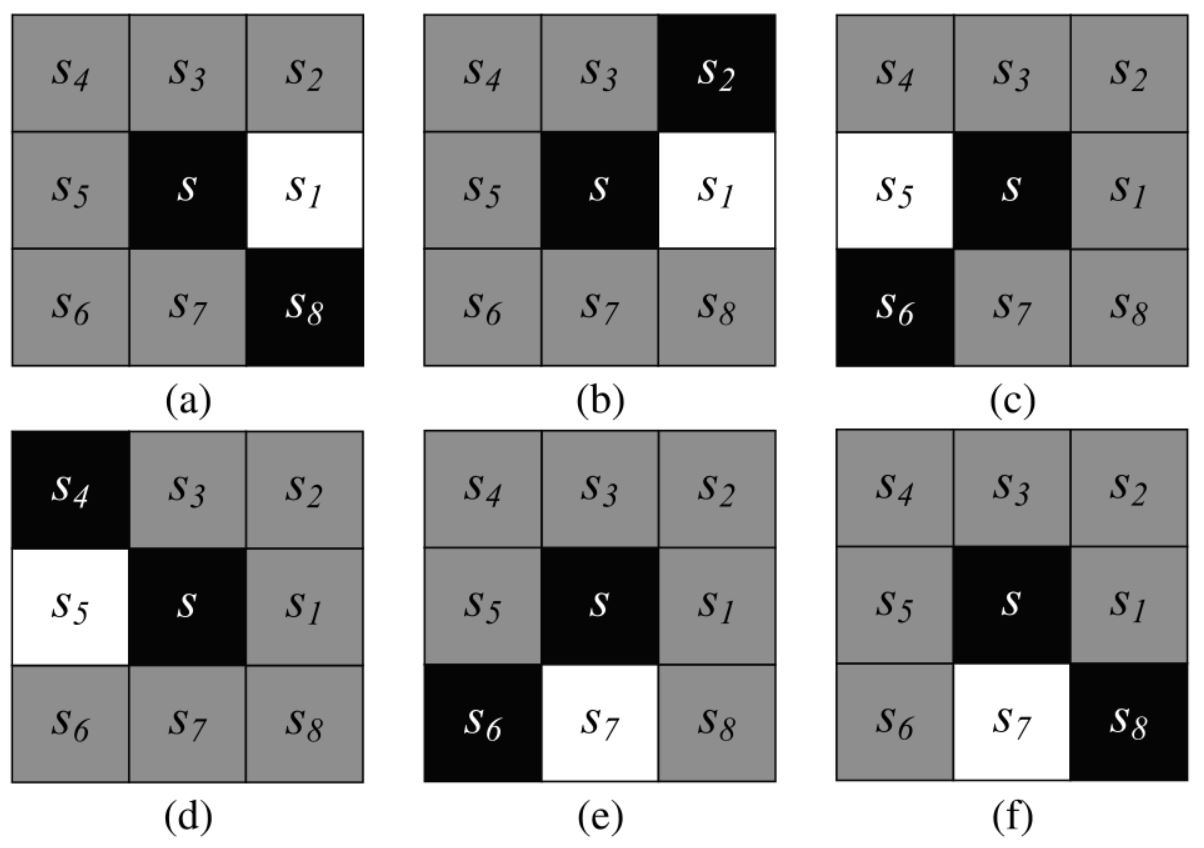
\includegraphics[width=0.5\textwidth]{fig/ccpp/bps}
	\caption[Conditions for backtracking points.]{Conditions for backtracking points \citep{Viet2013}. White tiles are free, black tiles are either covered or obstacle, gray tiles can be anything.}
	\label{fig:bps}
\end{figure}

The approach of \citet{Viet2013} assumes that one cell represents the coverage of a vacuum cleaner. However, the proposed method of this thesis assumes a varying coverage range sensor, and the proposed square cell partitioning allows multiple cells to be marked as covered. Thus, the backtracking point should be adjusted so that the distance between the new lap and the closest lap is twice the shortest coverage range of the latter.

\subsection{Planning a path to the backtracking point}

Planning a path from the critical point to the backtracking point can be done with a shortest path searching algorithm. The A* algorithm is a popular choice in robotic applications, and a description of the algorithm can easily be found online \citep{wiki:a_star}. By performing the search exclusively over free and already covered cells, the resulting path is guaranteed free of static obstacles. If it is discovered that a moving obstacle has obstructed the backtracking path, a new backtracking point is determined and the path is replanned from the current position. 

A* traverses the partitioned grid map one cell at a time. The low resolution of the cells will therefore lead to a path that is longer and has more turns than necessary. Inspired by \citet{Viet2013}, a smoothing of the path is done by removing the cells between any two cells with line-of-sight. Determining line-of-sight between two cells can be done by using the supercover line algorithm introduced for the square cell partitioning in Section \ref{sec:square_partition}. Line-of-sight is then achieved if none of the tiles intersected by the supercover line is an obstacle. The algorithm for smoothing the A* path is described in \citet{Viet2013}. \figref{fig:backtracking} shows the difference between a smoothed and non-smooth backtracking path. The resulting online CCPP algorithm is summarized in Algorithm 3.

%\todo[inline]{TODO: The backtracking point at the top of the map is the closest. Change figure.}

\begin{figure}[h!]
    \centering
	\makebox[\linewidth][c]{
	\begin{subfigure}[b]{0.5\textwidth}
		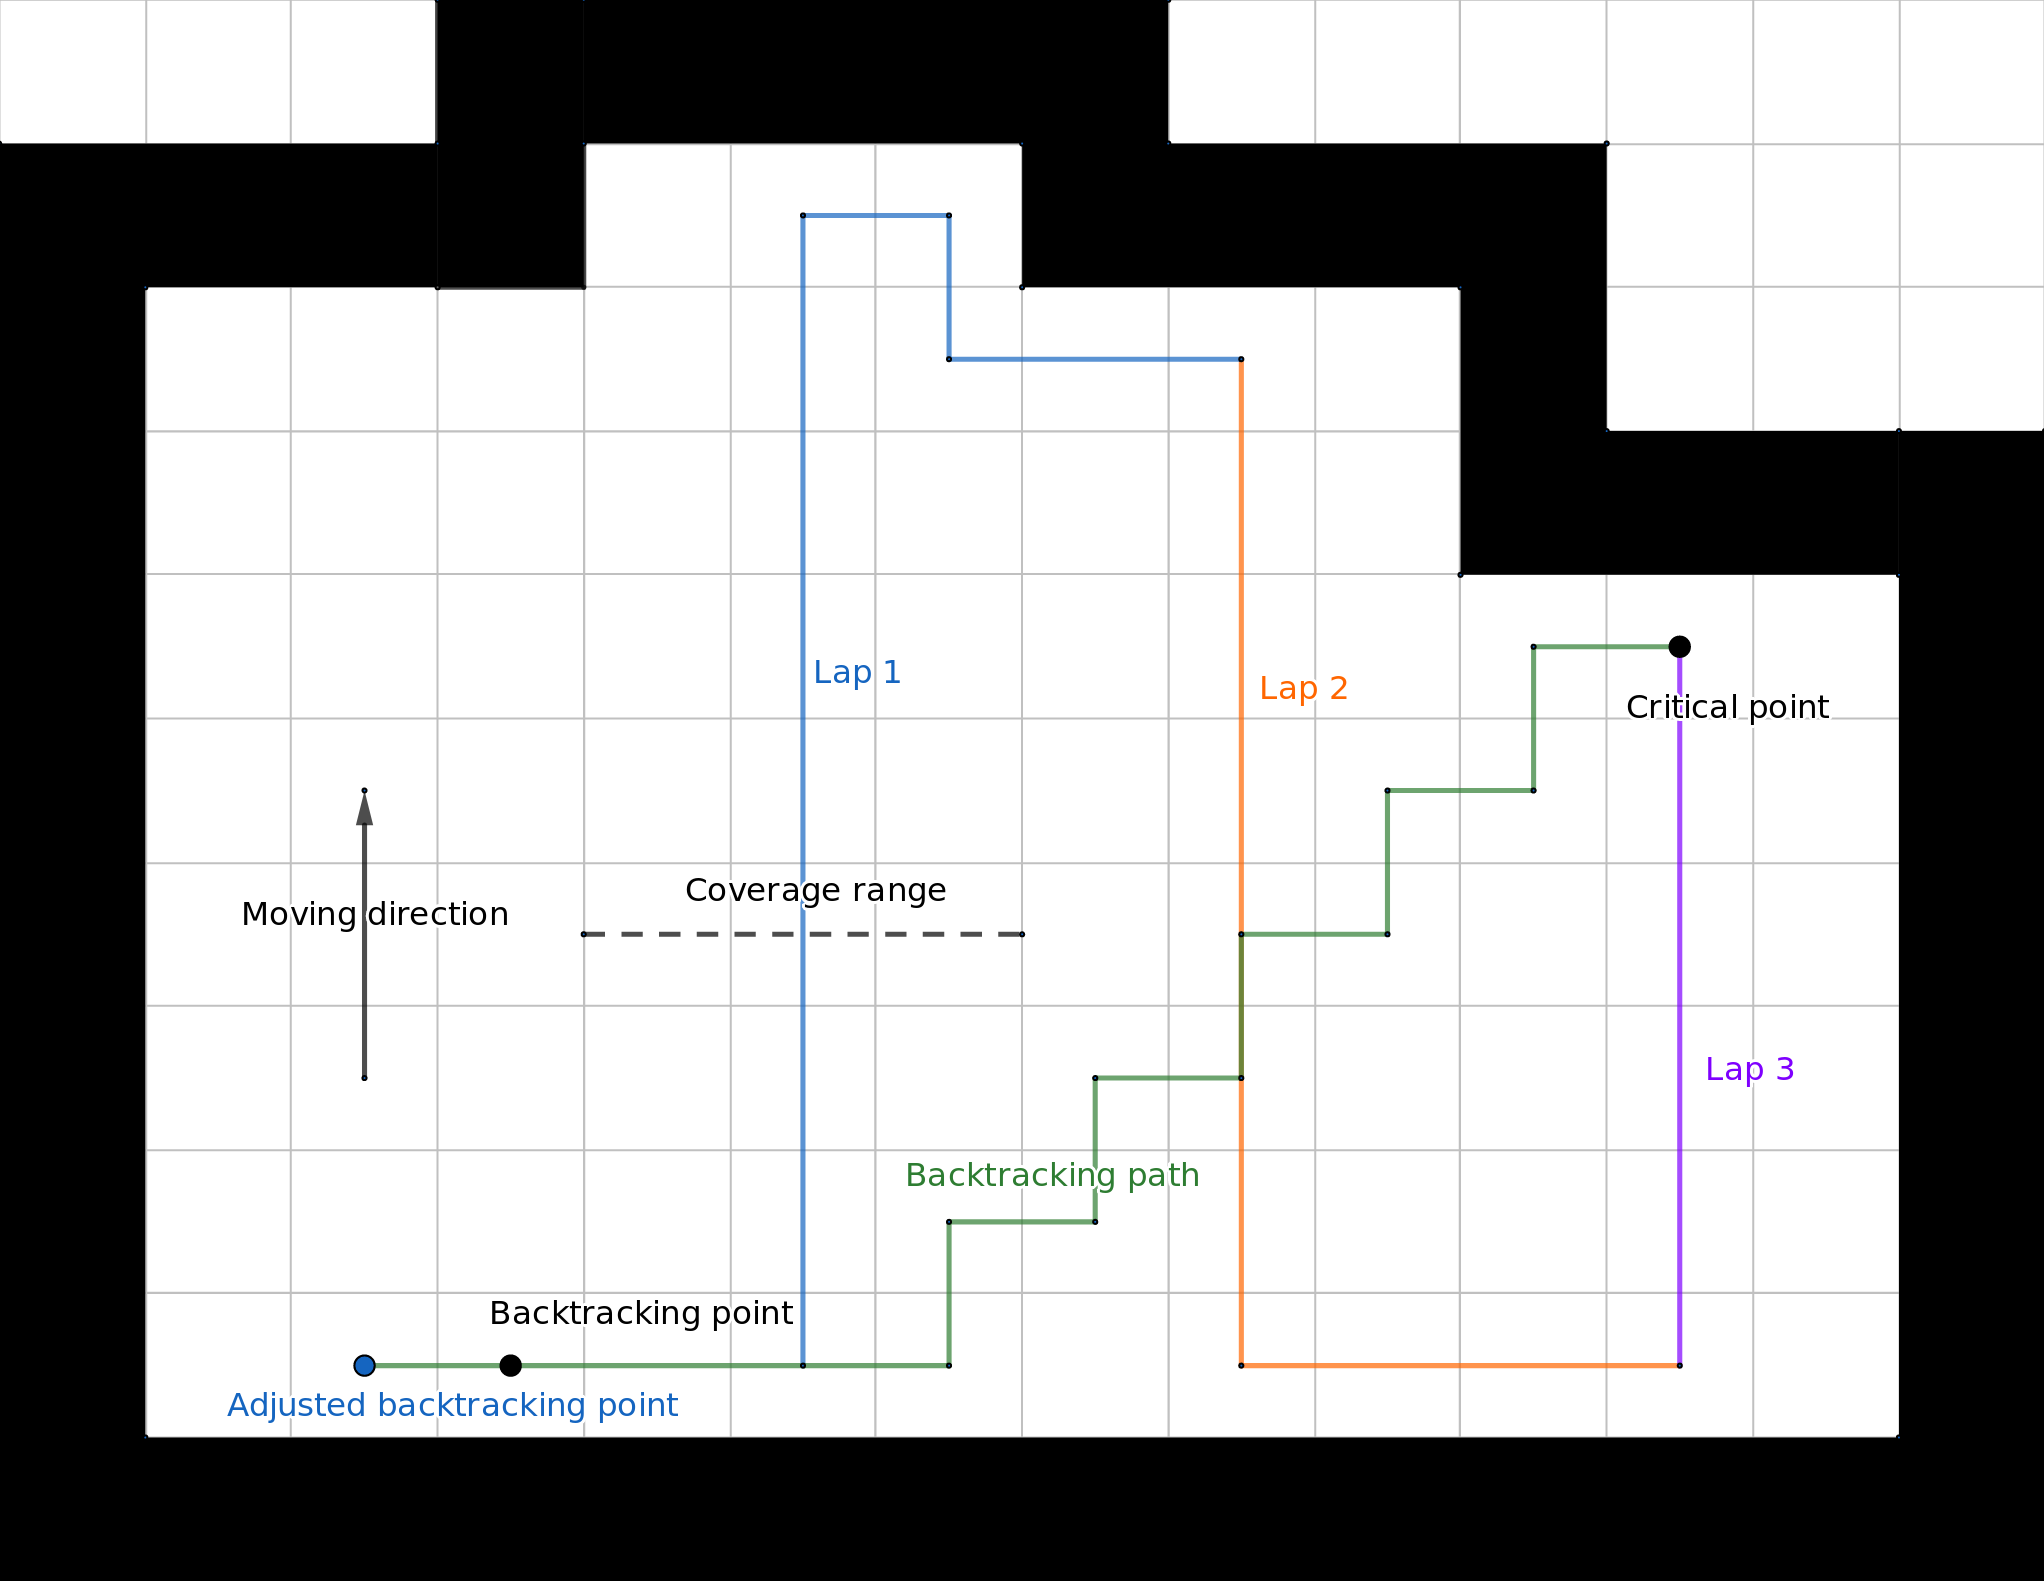
\includegraphics[width=1\linewidth]{fig/ccpp/backtracking_2}
		\caption{}
	\end{subfigure}
	\begin{subfigure}[b]{0.5\textwidth}
		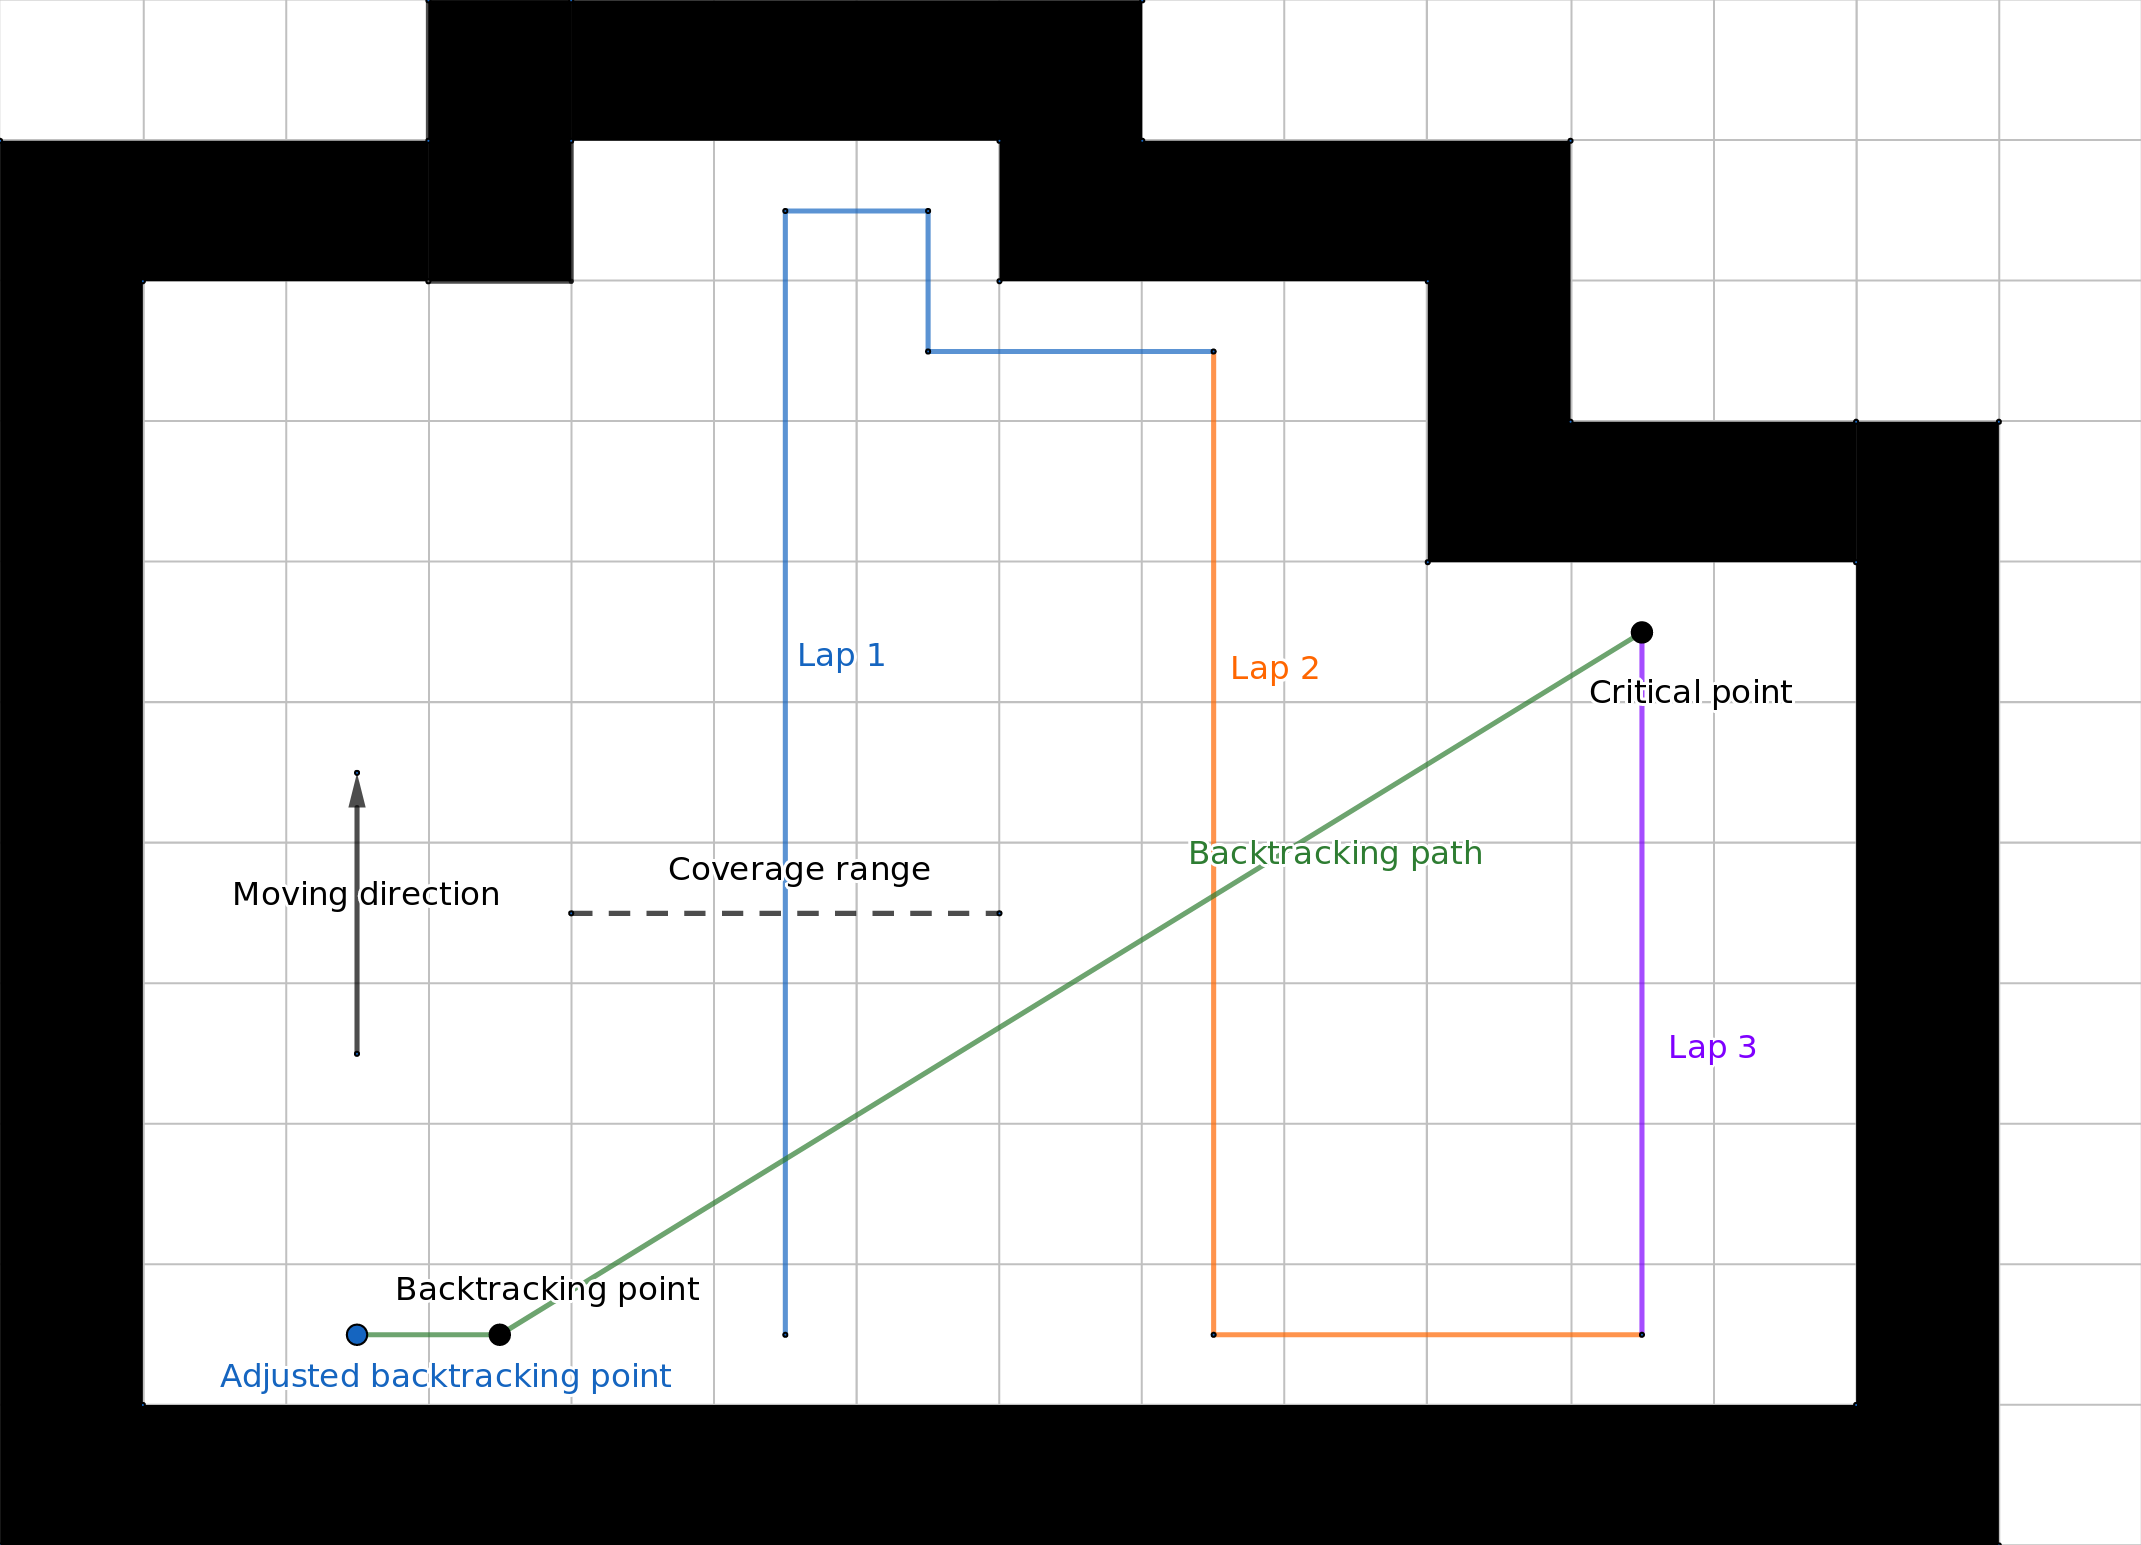
\includegraphics[width=1\linewidth]{fig/ccpp/backtracking_1}
		\caption{}
	\end{subfigure}
	}
	\caption[Smoothing of the A* backtracking path.]{A* smoothing. White cells are free and black cells are obstacles. (a) A non-smooth A* backtracking path. (b) The backtracking path is smoothed by removing cells between other cells with line-of-sight.} \label{fig:backtracking}
\end{figure}

\begin{tcolorbox}

\textbf{Algorithm 3: CCPP with boustrophedon motions}

\emph{Input: Pose of USV, and rolling window map }

\begin{enumerate}
\itemsep0em

\item Partition the workspace into square cells as described in Section \ref{sec:square_partition}. Set the status of each cell to unknown, and mark all cells as uncovered.

\item Begin to cover the workspace with a boustrophedon motion as described in Algorithm 2. The boustrophedon motion is finished when the algorithm arrives at a critical point.

\item With the accumulated knowledge from step 2, detect backtracking points according to \eqref{eq:bp1} and \eqref{eq:bp2}. If no backtracking points are found, complete coverage is achieved. Terminate the algorithm. Else, continue with the next step.

\item Determine the best backtracking point by finding the point requiring the shortest A* path. Apply line-of-sight smoothing to the shortest path.

\item Follow the smoothed A* path to the next starting point. Replan if it becomes blocked. Go to step 1.

\end{enumerate}

\end{tcolorbox}


